\documentclass[tikz,border=5pt]{standalone}

\usepackage{tikz}
\usetikzlibrary{positioning,arrows.meta,fit}

\begin{document}

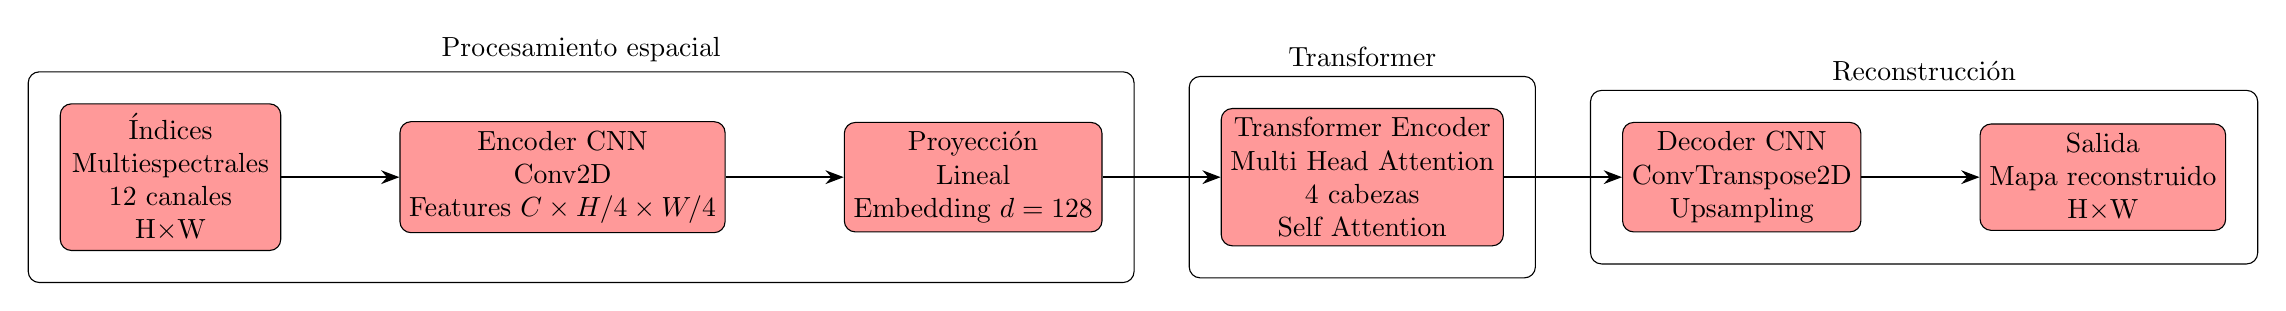
\begin{tikzpicture}[
node distance=1.5cm,
block/.style={
draw,
rounded corners,
minimum width=2.8cm,
minimum height=1.2cm,
align=center,
fill=red!40
},
arrow/.style={
->,
>=Stealth,
thick
}
]


% Input
\node[block] (input)
{
Índices\\
Multiespectrales\\
12 canales\\
H$\times$W
};


% Encoder
\node[block,right=of input] (enc)
{
Encoder CNN\\
Conv2D\\
Features $C\times H/4\times W/4$
};


\node[block,right=of enc] (proj)
{
Proyección\\
Lineal\\
Embedding $d=128$
};


% Transformer
\node[block,right=of proj] (att)
{
Transformer Encoder\\
Multi Head Attention\\
4 cabezas\\
Self Attention
};


% Decoder
\node[block,right=of att] (dec)
{
Decoder CNN\\
ConvTranspose2D\\
Upsampling
};


\node[block,right=of dec] (out)
{
Salida\\
Mapa reconstruido\\
H$\times$W
};



% arrows
\draw[arrow] (input)--(enc);
\draw[arrow] (enc)--(proj);
\draw[arrow] (proj)--(att);
\draw[arrow] (att)--(dec);
\draw[arrow] (dec)--(out);


% grupos

\node[
draw,
rounded corners,
fit=(input)(enc)(proj),
inner sep=0.4cm,
label=above:{Procesamiento espacial}
] {};


\node[
draw,
rounded corners,
fit=(att),
inner sep=0.4cm,
label=above:{Transformer}
] {};


\node[
draw,
rounded corners,
fit=(dec)(out),
inner sep=0.4cm,
label=above:{Reconstrucción}
] {};


\end{tikzpicture}

\end{document}